\documentclass[preprint]{aastex62}
\usepackage{graphicx}
\usepackage{amsmath}
\usepackage{natbib}
%\usepackage{subcaption}
\bibliographystyle{aasjournal}
\usepackage[version=4]{mhchem}

\begin{document}

\title{AST443 - Lab 0 - Properties of CCD Cameras}
\author{110508748}
%\date{}							% Activate to display a given date or no date

% General Guidelines
  % Write it like a scientific paper
  % Every sentence is precise and meaninful
  % Write with good English
  % UNDERSTAND the analysis and make that clear
  % Contain all information necessary to reproduce my analysis and results
  % Be concise
  % If you find yourself repeating sentences, consider making a table
  % Make sure there's a red thread
  
  % Figures
    % Ensure they're legible when printed out
    % Contain information 
    % Make sure the figure caption describes the figure adaquately
    % Make sure your results are reported in the body of the text, not just shown in a figure

\begin{abstract}
  % The abstract contains a summary of the paper.
  % A brief description of your observations
  % Your results!
  % Gets the point across
  % Good understanding of the subject and of your results
  % NOT lengthy introduction to the problem. No sentences like 'the aim was to learn about CCDs'. No information not in the main body of the paper
  
  Type Ia Supernovae are some of the most important astronomical events in the universe as they serve as yard sticks that are light years long for observational astromers. However, a paper by Ken Shen and Lars Bildsten reveals that the simulations which make these yard sticks so valuable are not fully developed and may be leading to inaccuracies in measurements \citep{shenNbildsten}. This report details the process by which nuclear astrophysics codes like Pynucastro, Microphysics, and Castro are used to test the claims of Shen \& Bildsten by simulating Type Ia Supernovae. It was found that... % gotta fill that in one in when I get results. 
  
  % Perhaps one last sentence here. -AB

\end{abstract}

\pagebreak

\section{Introduction}

  % Serves as a review of the subject of the paper
  % Needs to discuss and cite the appropriate literature 
  % Good understanding of the subject and of your results

  Supernovae (SNe), the explosive deaths of stars, are some of the most spectacular events in the universe. A special kind of supernovae, the Type Ia Supernovae, is especially notable for its use as an astronomical measure of distance. Type Ia supernovae occur when two stars are in orbit around each other where at least one star has already died once and has become a white dwarf (WD), usually with a mass around that of our sun ($M_{\odot}$). Material in the outer shells of the WD's partner can be stolen by the WD through its gravitational field. Once the WD has taken enough material to reach a mass of 1.4 times $M_{\odot}$, it explodes. This 1.4$M_{\odot}$ is called the Chandrasekhar mass. The explosion releases light of many colors and other wavelengths. The graph plotting how bright each wavelength of light is in the explosion is the spectrum. Since these stars usually have the same mass and elemental composition when they explode, the explosions have the same brightness and uniquely Type Ia SNe spectrum. 
  
  An observational astronomer can observe an event resembling a Type Ia SNe and use its spectrum to confirm it is a Type Ia Supernovae. The astronomer can then take the brightness of the explosion and use it to calculate how far away the supernovae is. By using Type Ia SNe in other galaxies to measure how far away they are along with other measurements, observational cosmologists have been able to measure the rate at which our universe is expanding. Without accurate models of Type Ia SNe, these calculations would not be possible. 
  
  The dilemma is that not all Type Ia Supernovae wait until their mass reaches  the Chandrasekhar mass of 1.4$M_{\odot}$ before they explode. Some explode at lower masses, in the subChandra range where their mass is less than 1.4$M_{\odot}$. This means the overall brightness and the spectrum of the explosion is slightly different from the Chandrasekhar mass Type Ia Supernovae. If an observational astronomer uses a subChandra Type Ia supernovae to measure distance, they will calculate a larger distance if they assume it is a Chandrasekhar mass star. This means, as computational nuclear astrophysicists, we need to model subChandra Type Ia SNe to help the observational astronomers make accurate calculations of astronomical distance. This has been done before, however, a paper by Ken Shen and Lars Bildsten has pointed out that previous simulations have not included as many possible nuclear reactions as it should have to make the calculations accurate \citep{shenNbildsten}. In this thesis I discuss the methods by which we use a computer code to simulate Type Ia SNe with the elements suggested by Shen and Bildsten. 

\section{Codes}

  \subsection{GitHub}
  	
    GitHub is a website used to mediate code sharing and code collaboration. Most of the codes discussed in this report are available online, with all code available for viewing, editing, and using (also known as open-sourced software). 

  \subsection{Pynucastro}
    
    Pynucastro is an open-sourced coding package developed by Dr. Michael Zingale and Dr. Donald Willcox to create networks of nuclear reactions that can be used in their simulations \citep{pynucastro}. It does so by collecting information on the rate at which nuclear reactions occur at different temperatures from a database called the JINA Reaclib Database. The formatted reaction rates are compiled into a network that can be access by simulations like Microphysics and Castro. 
  
  \subsection{Microphysics}
  
    Microphysics is an open-sourced software, available on the StarKiller GitHub repository, with routines designed to incorporate aforementioned networks of reaction rates into astrophysical simulations \citep{Microphysics}.
    It is equipped with unit tests designed to run stellar simulations in a short amount of time to troubleshoot problems on a small scale before promoting the simulations to a larger scale operation. Microphysics comes with some preexisting networks but can also use new networks generated by Pynucastro. 
  
  \subsection{Castro}
  
    Castro is an open sourced software, available under the AMReX-Astro repository on GitHub, and is designed to run full scale simulations of astrophysical events in one dimension, two dimensions, and three dimensions \citep{castro}. Simulations include Type Ia SNe, core collapse SNe, and WD mergers. 
  
\section{Motivation}
  
  As previously mentioned, Type Ia SNe are critical to measuring large astronomical distances. Observational astronomers rely heavily on accurate estimations for what they observe to make scientific claims to their data. In a 2009 paper by Lars Bildsten and Kenneth Shen, they theorized that the three elements used to simulate Type Ia supernovae were not enough to accurately simulate the spectra and light curve of a Type Ia supernovae \citep{shenNbildsten}. Additionally, not all Type Ia SNe occur when the WD becomes a total of 1.4 $M_{\odot}$, sometimes the explosions are set off, they detonate, before the Chandrasekhar mass is reached. This means that they could have different observational signatures that Chandrasekhar mass Type Ia SNe. It is critical that accurate models of Type Ia SNe are obtained in order for observational astronomers to learn about the universe accurately. 
  
  The goal for this research is to first create a nuclear reaction network following Shen and Bildsten's guidelines, test the network in Microphysics to see if there is a substantial change, then to run a model without the elements and reactions suggested by Shen \& Bildsten to be compared with a model that does consider their recommendations. If the change in results is drastic, then we will have more science to do. 
  
\section{Simulations and Results}
  
  \subsection{Pynucastro}
    
    {\tt Aprox13} is a nuclear reaction network composed of 13 element isotopes. It begins with Helium (\ce{^4He}, also known as an $\alpha$ particle) adds two \ce{^4He} to get a Carbon (\ce{^{12}C}) and one photon ($\gamma$) then continues to add $\alpha$ particles until Iron (\ce{^{56}Fe}) and a lot more $\gamma$'s are obtained. Since each isotope is connected by an $\alpha$ particle, this is called an $\alpha$ chain and earns the name 13 from the 13 isotopes on the $\alpha$ chain that it possesses. All elements that are \ce{^{24}Mg} and heavier are also connected through a process where an $\alpha$ particle hits an isotope and creates a new particle but kicks out a proton, then a different proton hits the new nucleus and one of those $\alpha$ chain isotopes are created along with a $\gamma$. In total the {\tt aprox13} network contains 22 isotopes and has proven to be a good model of stellar evolution, but Shen \& Bildsten suggest developing the reaction network more for Type Ia SNe \citep{timmes}.
    
    This study began through the use of Pynucastro to create the {\tt subch} network, standing for sub-Chandrasekhar. The network is composed of 8 reactions and 11 isotopes, with Chemical Equations  \ref{chemeq:1.1}, \ref{chemeq:1.2}, \ref{chemeq:2.1}, \ref{chemeq:2.2}, and \ref{chemeq:3.2} being the ones suggested by \citet{shenNbildsten} and the remaining three being a part of the $\alpha$ chain processes.
        
    \begin{align}
            \ce{3 ^4He &->  ^{12}C + 2\gamma } \\ 
            \ce{^{12}C + ^4He &->  ^{16}O + \gamma } \\
            \ce{^{14}N + ^4He &->  ^{18}F + \gamma } \label{chemeq:1.1} \\
            \ce{^{18}F + ^4He &-> ^{21}Ne +  p+} \label{chemeq:1.2} \\
            \ce{^{12}C + p+ &-> ^{13}N + \gamma } \label{chemeq:2.1} \\
            \ce{^{13}N + ^4He &-> ^{16}O + \text{p}} \label{chemeq:2.2} \\ 
            \ce{^{16}O + ^4He &-> ^{20}Ne + \gamma } \\
            \ce{^{14}C + ^4He &-> ^{18}O + \gamma } \label{chemeq:3.2}
    \end{align}
  
  \subsection{Microphysics}
  
    This new network is now used in Microphysics. There is a unit test in Microphysics referred to as {\tt burn\_cell} which simulates the chemical evolution in one small zone of a star. This test is first used to determine what tolerance will optimize results and reduce computation time in this simulation. Using these results, the {\tt burn\_cell} test will be used to simulate the chemical evolution of this zone as nuclear reactions take place to use and generate different elemental isotopes. 
  
    \subsubsection{Testing Simulation Equation Tolerances}
  
      Tolerances are parameters used to gauge how accurately the equation solvers in the simulation are doing their job. A smaller tolerance typically leads to a more precise answer but takes more computer time. For this reason, a tolerance of $10^{-12}$ was treated as an exact answer and the tolerances of $10^{-3}$, $10^{-6}$, and $10^{-9}$ were tested. 
     
      To test these tolerances, a fraction of  \ce{^4He}, \ce{^{12}C}, and \ce{^{16}O} were initialized in one zone as modeled by the {\tt burn\_cell} unit test. The zone is heated so that the three elements begin to burn with each other. Simulations are run with a tolerance of $10^{-3}$, $10^{-6}$, $10^{-9}$, and $10^{-12}$ in a zone that is initialized to a temperature of 0.3 billion Kelvin with a density of one million grams per cubic centimeter. The relative error in each element's mass fraction, $X$, is calculated between the 3 former simulations and the $10^{-12}$ simulation, as defined by 
    
      \begin{equation}
        \sigma_X = \frac{X_{10^{-12}} - X_{\text{former}}}{X_{10^{-12}}} \text{    , }
        \label{eq:relativeerror}
      \end{equation}
    
      for each point in time during the simulation. This relative error in mass fraction is plotted as a function of time for each of the three testing simulations and can be seen in Figure~\ref{fig:relativeerror}.
    
      \begin{figure}
        \centering
        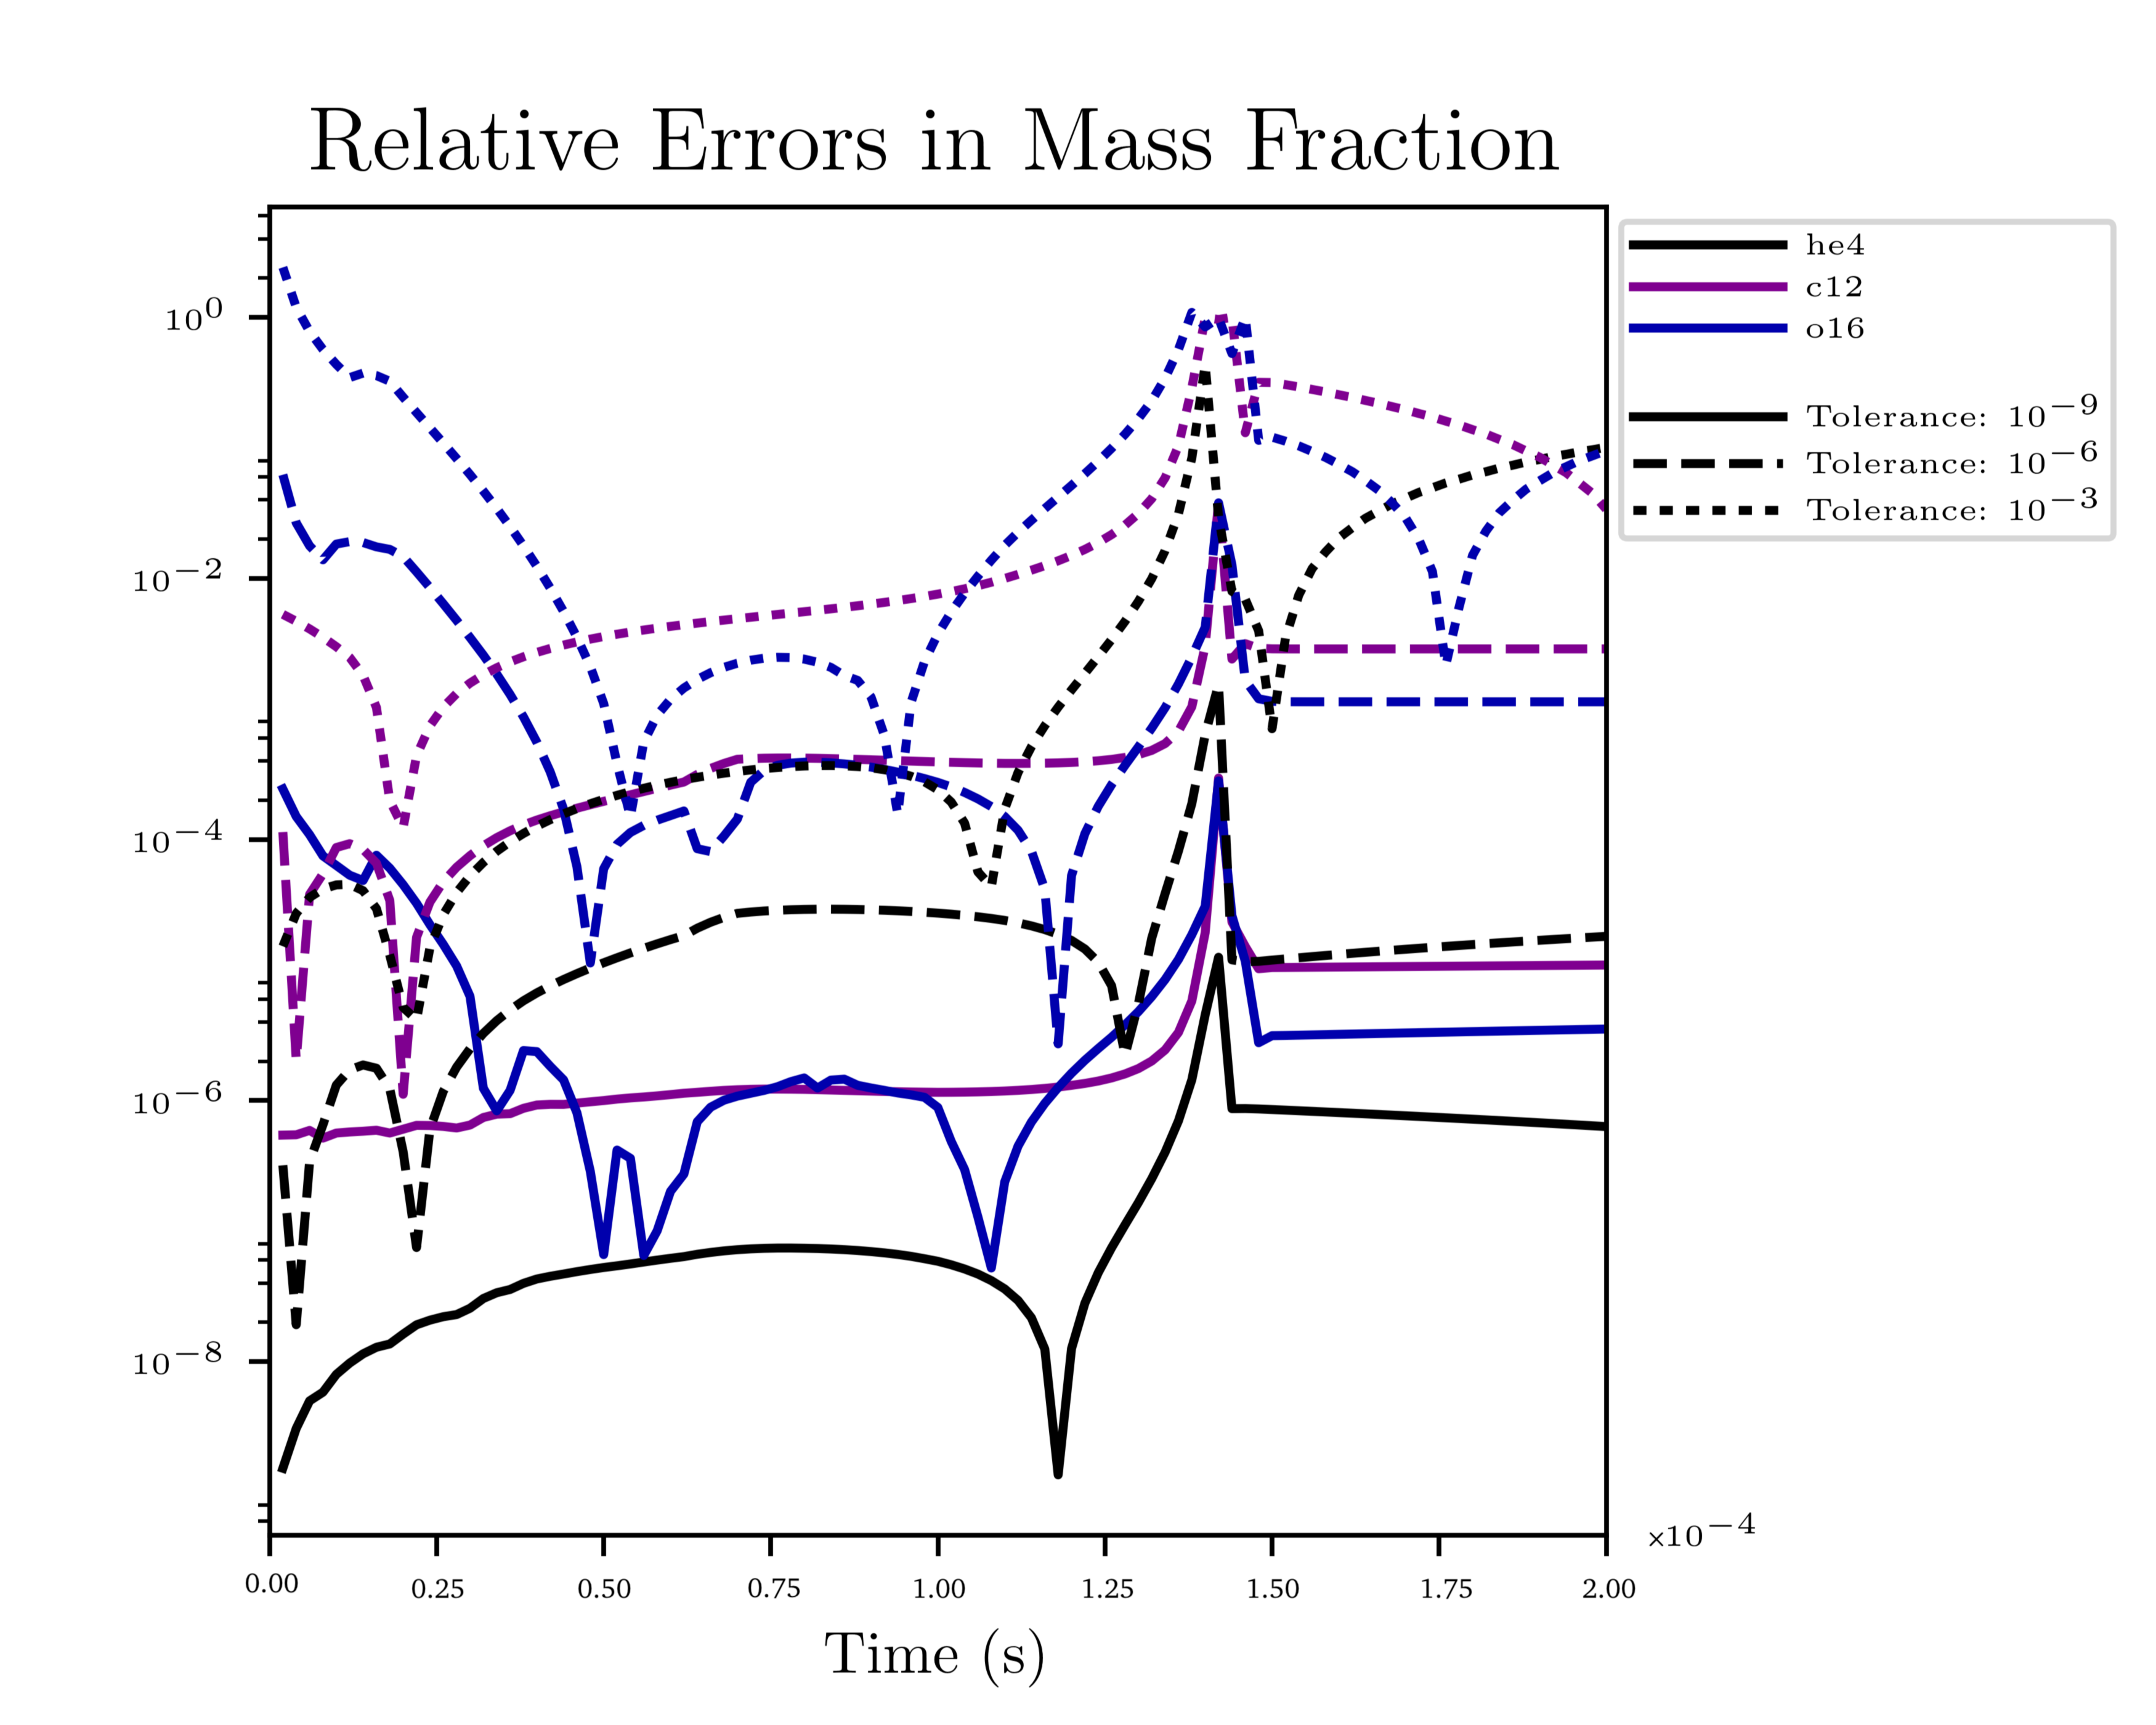
\includegraphics[width=5in]{images/react_aprox13_test13_ureca_tol-rel_xn1.png}
        \caption{Relative error over time of the \ce{^4H} (in black), \ce{^{12}C} (in purple), and \ce{^{16}O} (in blue) mass fractions run in simulations with a tolerance of $10^{-9}$ (solid line), $10^{-6}$ (dashed line), and $10^{-3}$ (dotted line) calculated with respect to the true values calculated by a simulation with a tolerance of $10^{-12}$. The lower the value, the closer the result is to the true value.
          }
        \label{fig:relativeerror}
      \end{figure}  
  
      From Figure~\ref{fig:relativeerror}, one can see that the solid lines, corresponding with the simulation using a tolerance of $10^{-9}$, are consistently the lowest. The relative error of the simulation with a tolerance of $10^{-9}$ is consistently below $10^{-3}$ and drops as low as $10^{-8}$ at times without taking much longer to run than the simulations with tolerances of $10^{-6}$ and $10^{-3}$. Therefore, it is concluded that a tolerance of $10^{-9}$ is acceptable for the codes going forwards. 
  
    \subsubsection{Using Mass Fraction Evolution to Justify Motivation}
    
      The next step with the {\tt burn\_cell} tests is to test if the {\tt subch} network is producing results worth investigating. The main ingredients to the simulation that Shen \& Bildsten encouraged were \ce{^{14}C} and \ce{^{14}N} \citep{shenNbildsten}. Figure~\ref{fig:microphysicsX} shows the time evolution of mass fractions, $X$, for each of the eleven isotopes in the {\tt subch} network for three different {\tt burn\_cell} simulations. This zone, too, is initialized at a temperature of 0.3 billion Kelvin and a density of one million grams per cubic centimeter. One simulation is run without \ce{^{14}C} and \ce{^{14}N}, one with some \ce{^{14}N}, and the last with both \ce{^{14}C} and \ce{^{14}N}. If this Shen \& Bildsten's theory is correct, we shouldn't see 11 clean and solid lines, but many more dotted and dashed lines that show there is a change in each of the simulations. In Figure~\ref{fig:microphysicsX}, seeing a combination of solid, dashed, and dotted lines at different orders of magnitudes for many elements implies that the incorporation of \ce{^{14}C} and \ce{^{14}O} is important. 
      
      \begin{figure}
        \centering
        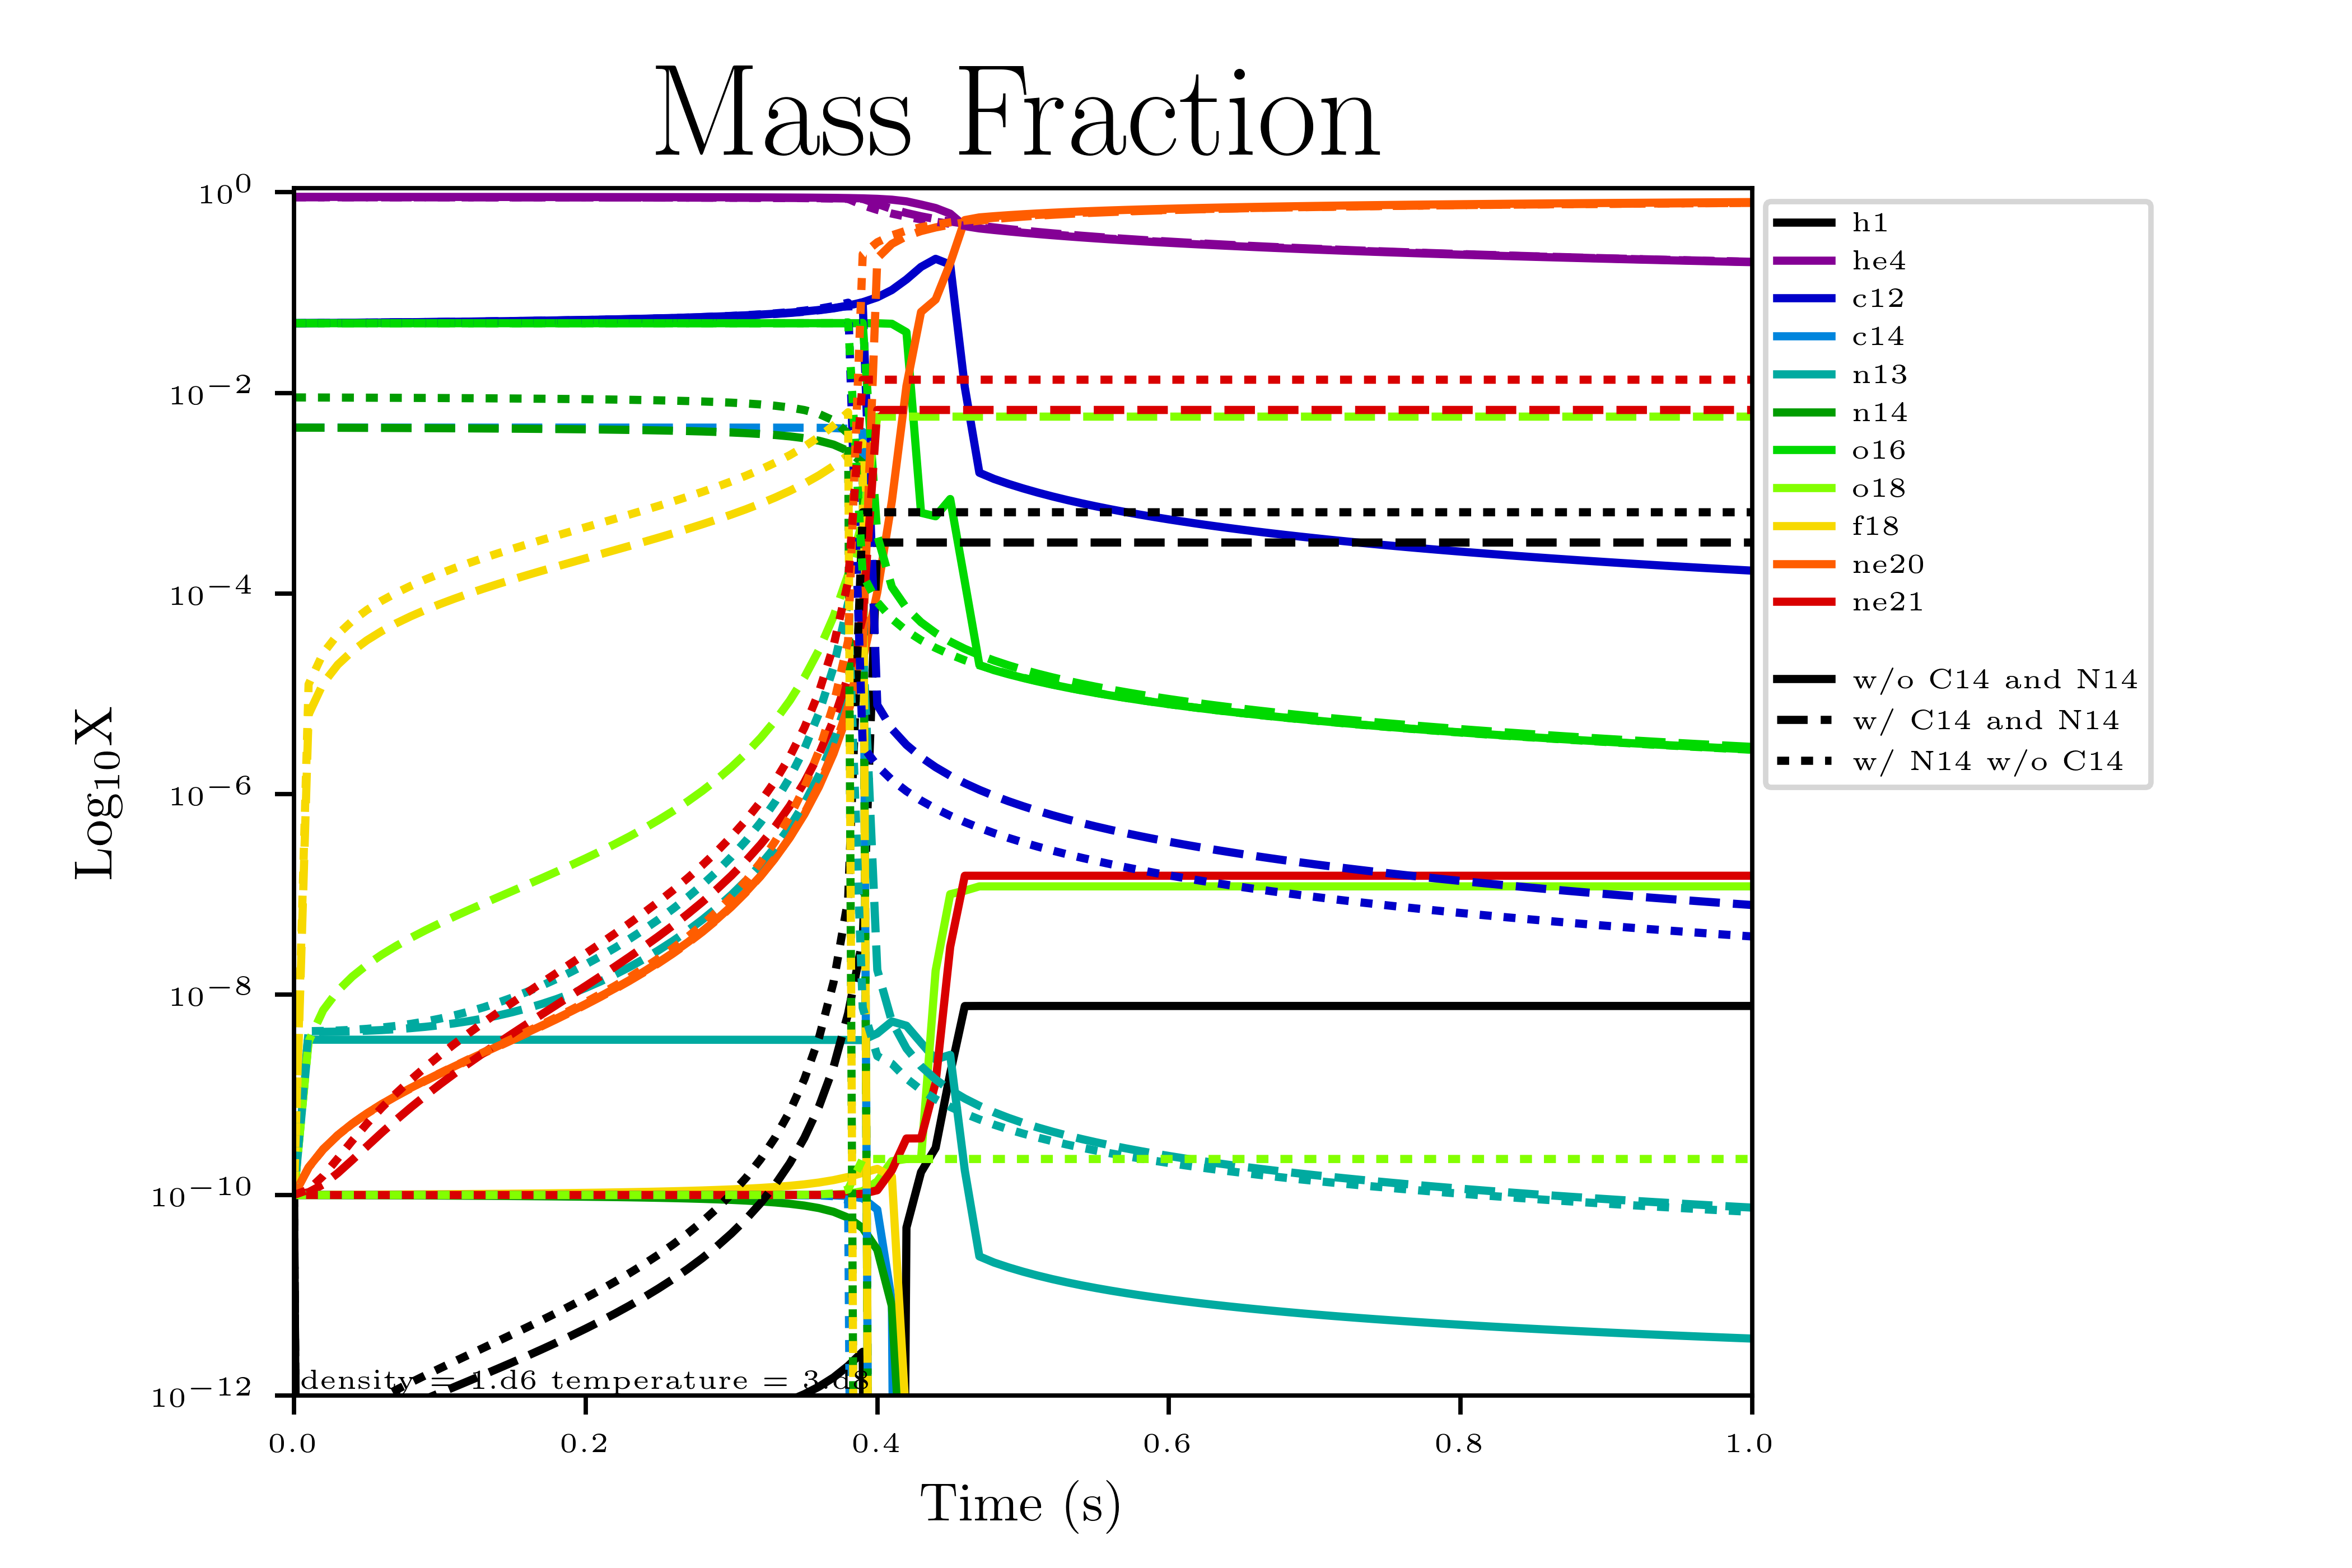
\includegraphics[width=6in]{images/subch_nC14nN14_xn_tol-10.png}
        \caption{Mass fraction, $X$, evolution over time for the 11 elements (differentiated by color) in the {\tt subch} network for three different {\tt burn\_cell} simulations: one without \ce{^{14}C} and \ce{^{14}O} (solid lines), one with both \ce{^{14}C} and \ce{^{14}O} (dashed line), and with \ce{^{14}O} but no \ce{^{14}C} (dotted line). Notice the large change in \ce{^{12}} and \ce{^{21}} between the simulations.
          }
        \label{fig:microphysicsX}
      \end{figure} 
      
      In addition to the mass fraction evolution, the rate of energy generated by the zone in the {\tt burn\_cell} simulation is plotted as a function of time in Figure~\ref{fig:energygeneration}. Once more, this is done for a simulation without \ce{^{14}C} and \ce{^{14}N}, adding only \ce{^{14}N}, and adding both \ce{^{14}C} and \ce{^{14}N}. From Figure~\ref{fig:energygeneration} one can see that in the simulations with \ce{^{14}C} and \ce{^{14}N}, the energy generated by this zone peaks sooner and has a lower peak.  This shows that when \ce{^{14}C} and \ce{^{14}O} are incorporated into the simulations of Type Ia SNe, they will generate energy faster, use their nuclear energy more quickly, and have a smaller maximum energy generation rate than simulations without these elements. This is another nudge in the direction of running a full scale simulation. 
      
      \begin{figure}
        \centering
        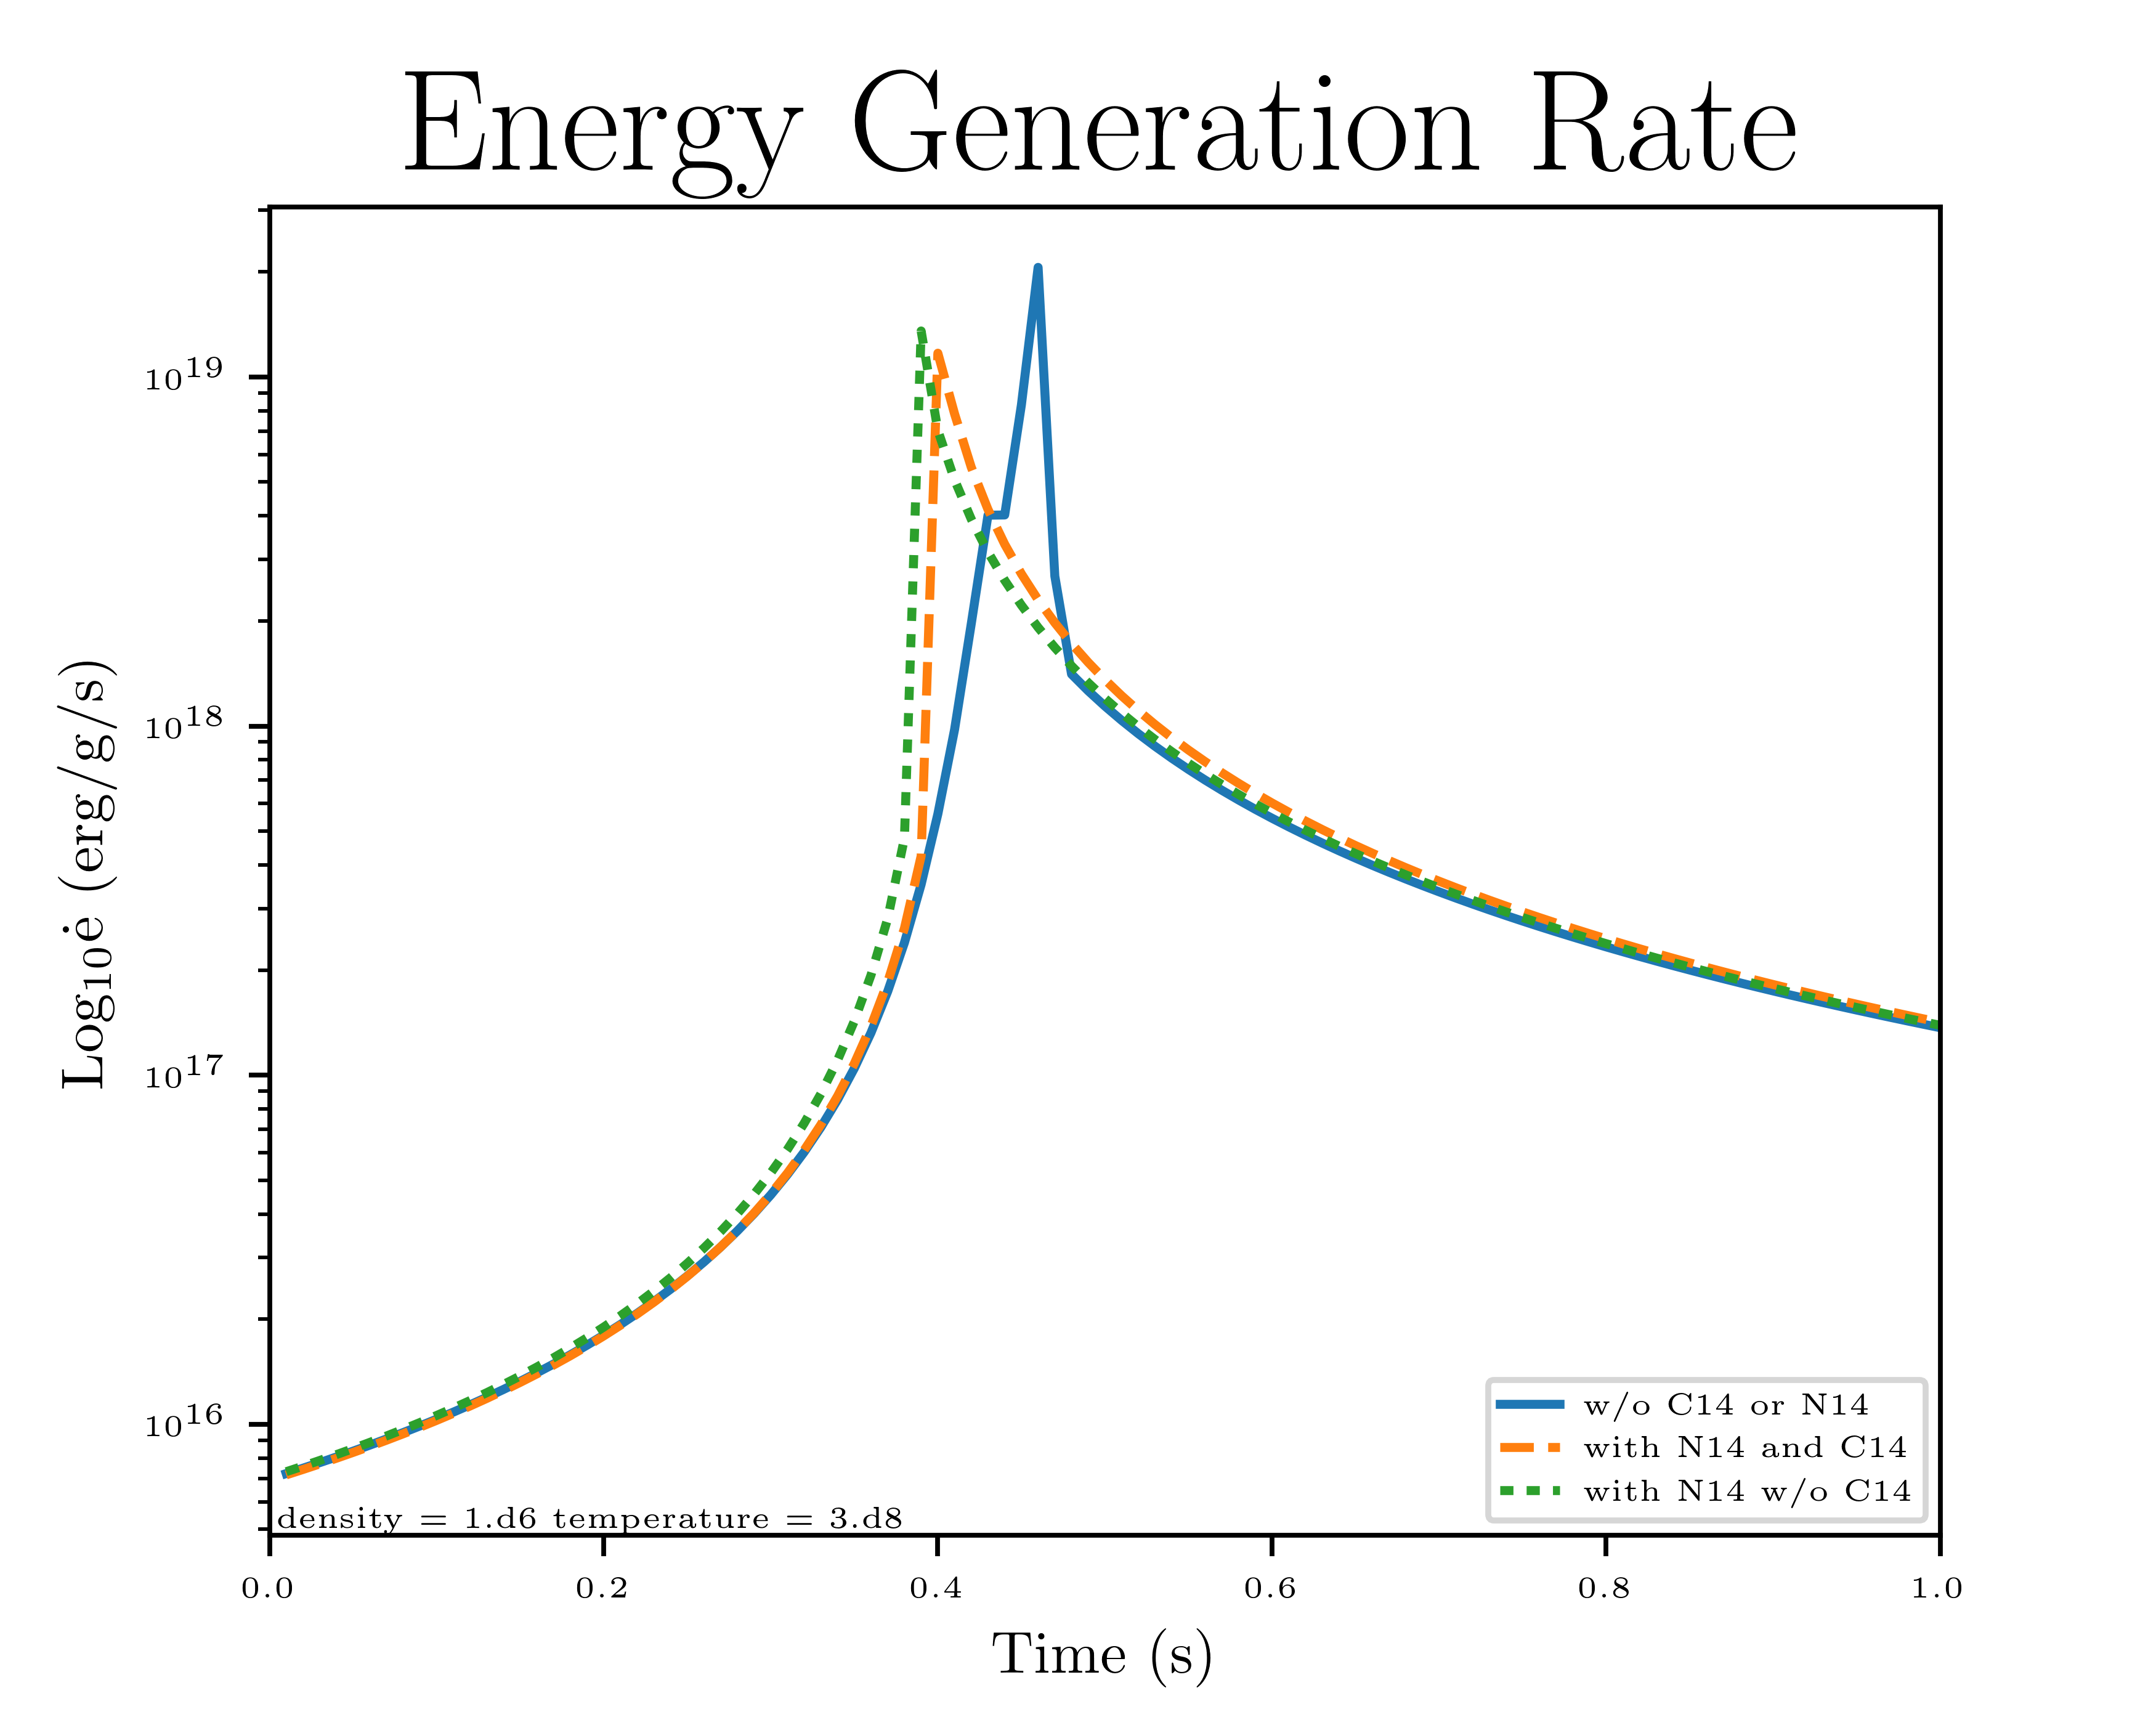
\includegraphics[width=5in]{images/subch_nC14nN14_edot_tol-10.png}
        \caption{The rate of energy generated by the zone in the {\tt burn\_cell} simulation as a function of time for the run without \ce{^{14}C} and \ce{^{14}O} (solid lines), with both \ce{^{14}C} and \ce{^{14}O} (dashed line), and with \ce{^{14}O} but no \ce{^{14}C} (dotted line).
          }
        \label{fig:energygeneration}
      \end{figure} 
      
\newpage
  
  \subsection{Multi-dimensional simulations with Castro}
  
    The Castro code will be used to first test the {\tt subch} network in one dimension to see if an increase in temperature will ignite a flame and push it across a layer of helium. If so, then the Castro code will be used to simulate the star in two dimensions. This can then be compared to simulations of stars using other networks and the results can be compared. 
    
    \subsubsection{1-Dimensional Simulations}
    
      Using the Castro science problem called "Detonation", a simulation of a flame propagating from left to right was initialized with the {\tt subch} network. The layer of helium that this flame is propagating through has a density of 1 million grams per cubic centimeter, has a flame with a temperature of 2 billion Kelvin (on the left), and has a resting temperature of 0.05 billion Kelvin (on the right). As shown in Figure~\ref{fig:detonation}, the energy released from nuclear reactions in the flame powers a wave to the right side of the screen and off of the page. 
      
    \begin{figure}
      \gridline{
        \fig{images/flame_subch_plt_0}{0.7\textwidth}{(a)}
        }
      \gridline{
        \fig{images/flame_subch_plt_110}{0.48\textwidth}{(b)}
        \fig{images/flame_subch_plt_520}{0.48\textwidth}{(c)}
        }
      \caption{The above images depict a flame wave (shown by a shelf of temperature on the left at 2 billion K) propagating in the right direction at the beginning of the simulation (Figure (a)), after 0.002 seconds (Figure (b)), and after 0.01 seconds (Figure (c)).}
      \label{fig:detonation}
    \end{figure}
      
      Now, knowing that a mild temperature perturbation can ignite a helium layer, this simulation can be taken to two dimensions, which is a big step. These one dimensional simulations take a couple minutes to run on an average computer but the two dimensional simulations will take much longer, even on a much larger computer. 
      
\newpage
    
    \subsubsection{2-Dimensional Simulations}
  
      The two dimensional simulations are completed by wrapping a \ce{^{12}C} and \ce{^{16}O} WD core in a thick layer of \ce{^4He} then taking a half moon shaped slice of the WD and simulating the two dimensional burning in this slice. The burning is initiated by a hot temperature perturbation at the interface between the helium shell and the core along the north pole of the star. 
      
      The zone of simulation is 1.25 billion centimeters wide by 2.5 billion centimeters high, 3 levels of refinement are used (more levels, more accurate, longer run time), a perturbation temperature factor of 80, a perturbation radius factor of 8, centered at a distace of 0.35 billion centimeters from the center from the star. Using the {\tt subch} network to simulate this, the images in Figure~\ref{fig:subchsims} resulted. 
      
      \begin{figure}
        \gridline{
          \fig{images/subch_20190412_plt00100_Temp_slice}{0.48\textwidth}{(a)}
          \fig{images/subch_20190412_plt122900_Temp_slice}{0.48\textwidth}{(b)}
          }
        \caption{These plots were created using {\tt amrvis} which can be found in the AMReX coding package \citep{AMREXcodes}. They depict the WD as a half circle in the left middle and use color to display the temperature in the plane. A redder color is a cooler temperature and a yellow color represents warmer temperatures. Note that the values associated with the color scale of the temperature may change between pictures. 
          }
        % PLEASE NOTE THAT THESE IMAGES ARE FROM APRIL AND ARE NOT UP TO DATE. THEY ARE PLACEHOLDERS. -AB
        \label{fig:subchsims}
      \end{figure}
      
      %Compare it to the aprox13 runs and talk about it. - AB

\section{Conclusion}

  % Summary of the analysis
  % Emphasis is on the results and their interpretation, and how they relate to results in the literature
  % Can provide an outlook, e.g. how the measurement can be improved with future measurements
  % Good understanding of the subject and of your results
  
  Shen \& Bildsten's paper brought light that simulations of Type Ia SNe needed more work, motivating the investigation narrated in this report. After checking the accuracy of codes used, simulations using a network of nuclear reaction rates based off of the Shen \& Bildsten paper were used in a one zone simulation, moving to a one dimensional simulation, and culminating in an insightful two dimensional simulation \citep{shenNbildsten}. It was proven that % fill this in when results exist. -AB
  
  The next steps moving forward will be to perform this in a three dimensional simulation. Using these results we can motivate fellow scientists to use their codes to retrieve the information about brightness curves and spectra so that observational astronomer can use them for calculating astronomical distance. Through the generation of better simulations, the scientific community gains better results and can produce excellent science. 

\bibliography{references}

\end{document} 